\documentclass[aspectratio=169]{beamer}

% Shared Beamer settings for Applied Machine Learning lectures (UPES).
% Keep this file free of \documentclass to allow reuse via \input.

% Allow lecture sources to use shared theme/assets without copying them into each lecture folder.
% NOTE: These paths are relative to `Unit-xx/Lecture-yy/latex/` (and `Lab/Experiment-xx/latex/`).
\makeatletter
\def\input@path{{../../../_shared/}{../../../_shared/UPES-Beamer-Theme/}}
\makeatother

\usetheme{UPES}
\setbeamertemplate{navigation symbols}{}

\usepackage{amsmath}
\usepackage{amssymb}
\usepackage{booktabs}
\usepackage{graphicx}
\usepackage{hyperref}
\usepackage{xcolor}
\usepackage{listings}

% Code listings (Python-oriented for this subject).
\lstset{
  language=Python,
  basicstyle=\ttfamily\small,
  keywordstyle=\color{blue},
  commentstyle=\color{gray},
  stringstyle=\color{teal},
  showstringspaces=false,
  columns=fullflexible,
  breaklines=true
}

\usepackage{tikz}
\usetikzlibrary{arrows.meta,positioning,shapes.geometric,calc,fit,backgrounds}

% Per-slide source line (references shown on the slide itself).
\newcommand{\slidesources}[1]{%
  \vfill
  {\tiny\color{gray}\raggedright\sloppy\parbox{\linewidth}{Sources: #1}\par}%
}

% Unit-wise source strings for this subject (used by slides/notes).
% Path is relative to the lecture `latex/` folder (the compilation CWD).
% Source strings for Applied Machine Learning (CSAI2017P) — used by slides + notes.
% Prescribed texts and reference books are taken from the course syllabus.
% Support texts are the author-hosted open-access editions:
%   statlearning.com            (ISL with Python)
%   probml.github.io/pml-book   (Murphy, Probabilistic Machine Learning)
%   d2l.ai                      (Dive into Deep Learning)
%   mml-book.github.io          (Mathematics for Machine Learning)

\newcommand{\AMLRepoURL}{https://github.com/tali7c/Applied-Machine-Learning}

% --- prescribed -------------------------------------------------------------
\newcommand{\AMLPrescribed}{%
M\"uller and Guido, \textit{Introduction to Machine Learning with Python}, O'Reilly, 2016.;%
Bishop, \textit{Pattern Recognition and Machine Learning}, Springer, 2006.;%
Murphy, \textit{Machine Learning: A Probabilistic Perspective}, MIT Press, 2012.;%
Han, Kamber and Pei, \textit{Data Mining: Concepts and Techniques} (3e), Morgan Kaufmann, 2012.%
}

% --- unit-wise ---------------------------------------------------------------
\newcommand{\AMLUnitISources}{%
M\"uller and Guido, \textit{Introduction to Machine Learning with Python}, Ch. 1.;%
Bishop, \textit{Pattern Recognition and Machine Learning}, Ch. 1.;%
Murphy, \textit{Probabilistic Machine Learning: An Introduction}, MIT Press, 2022, Ch. 1.;%
Mitchell, \textit{Machine Learning}, McGraw Hill, 1997, Ch. 1.;%
Scikit-learn documentation, accessed 2026-08-04.%
}

\newcommand{\AMLUnitIISources}{%
Bishop, \textit{Pattern Recognition and Machine Learning}, \S1.5, \S4.3, \S7.1.;%
Zhang, Lipton, Li and Smola, \textit{Dive into Deep Learning}, \S3.4.;%
Shalev-Shwartz and Ben-David, \textit{Understanding Machine Learning}, Ch. 15.;%
Murphy, \textit{Probabilistic Machine Learning: An Introduction}, Ch. 5.%
}

\newcommand{\AMLUnitIIISources}{%
Zhang, Lipton, Li and Smola, \textit{Dive into Deep Learning}, Ch. 12 (Optimization Algorithms).;%
Deisenroth, Faisal and Ong, \textit{Mathematics for Machine Learning}, Ch. 7.;%
Kingma and Ba, ``Adam: A Method for Stochastic Optimization,'' ICLR 2015.;%
Ruder, ``An overview of gradient descent optimization algorithms,'' arXiv:1609.04747, 2016.%
}

\newcommand{\AMLUnitIVSources}{%
Han, Kamber and Pei, \textit{Data Mining: Concepts and Techniques} (3e), Ch. 3.;%
M\"uller and Guido, \textit{Introduction to Machine Learning with Python}, Ch. 3--4.;%
James, Witten, Hastie, Tibshirani and Taylor, \textit{An Introduction to Statistical Learning with Python}, Ch. 5--6, 12.;%
Scikit-learn documentation (preprocessing, model selection), accessed 2026-08-04.%
}

\newcommand{\AMLUnitVSources}{%
James et al., \textit{An Introduction to Statistical Learning with Python}, Ch. 3--6.;%
Bishop, \textit{Pattern Recognition and Machine Learning}, Ch. 3.;%
Deisenroth, Faisal and Ong, \textit{Mathematics for Machine Learning}, Ch. 9.;%
M\"uller and Guido, \textit{Introduction to Machine Learning with Python}, \S2.3.%
}

\newcommand{\AMLUnitVISources}{%
Han, Kamber and Pei, \textit{Data Mining: Concepts and Techniques} (3e), Ch. 8--9.;%
James et al., \textit{An Introduction to Statistical Learning with Python}, Ch. 8--9.;%
Bishop, \textit{Pattern Recognition and Machine Learning}, Ch. 4--5, 7, 14.;%
Zhang et al., \textit{Dive into Deep Learning}, Ch. 5.%
}

\newcommand{\AMLUnitVIISources}{%
Han, Kamber and Pei, \textit{Data Mining: Concepts and Techniques} (3e), Ch. 10.;%
James et al., \textit{An Introduction to Statistical Learning with Python}, Ch. 12.;%
M\"uller and Guido, \textit{Introduction to Machine Learning with Python}, \S3.5.;%
Ester, Kriegel, Sander and Xu, ``A density-based algorithm for discovering clusters (DBSCAN),'' KDD 1996.%
}

\newcommand{\AMLLabSources}{%
M\"uller and Guido, \textit{Introduction to Machine Learning with Python}, companion notebooks.;%
McKinney, \textit{Python for Data Analysis} (3e), O'Reilly, 2022.;%
Scikit-learn user guide, accessed 2026-08-04.;%
Matplotlib and Seaborn documentation, accessed 2026-08-04.%
}



\graphicspath{{../figures/}{../images/}{../../../_shared/}{../../../_shared/UPES-Beamer-Theme/}}

\title[Applied Machine Learning]{Applied Machine Learning}
\subtitle{Unit 06 -- Lecture 17: Neural Networks and Backpropagation}
\author{Tofik Ali}
\institute{School of Computer Science, UPES Dehradun}
\date{Autumn 2026}

% ---- a compact "output" block so code and its result sit together ----------
\lstdefinestyle{outblk}{
  basicstyle=\ttfamily\scriptsize\color{black!75},
  backgroundcolor=\color{black!5}, frame=leftline, framerule=2pt,
  rulecolor=\color{black!30}, breaklines=true, columns=fullflexible,
  keepspaces=true,   % several outputs below are aligned tables
  language={},       % printed output is not Python: do not syntax-highlight it
  xleftmargin=4pt, aboveskip=1pt, belowskip=1pt, literate={-}{{-}}1}
\lstnewenvironment{outblk}{\lstset{style=outblk}}{}

\begin{document}

\UPESCoverFrame
\setcounter{framenumber}{0}

\begin{frame}
  \titlepage
  \begin{center}
    \footnotesize One equation, applied over and over: the chain rule\\[0.25em]
    \footnotesize Topic focus: \textbf{backpropagation, derived and checked}\\[0.25em]
    \footnotesize Repository: \texttt{\AMLRepoURL}
  \end{center}
  \slidesources{\AMLUnitVISources}
\end{frame}

\begin{frame}{Quick Links}
  \centering
  \hyperlink{sec:perc}{\beamerbutton{The perceptron}}\hspace{0.4em}
  \hyperlink{sec:xor}{\beamerbutton{XOR}}\hspace{0.4em}
  \hyperlink{sec:act}{\beamerbutton{Activations}}\hspace{0.4em}
  \hyperlink{sec:bp}{\beamerbutton{Backpropagation}}\\[0.6em]
  \hyperlink{sec:mlp}{\beamerbutton{Training an MLP}}\hspace{0.4em}
  \hyperlink{sec:init}{\beamerbutton{Initialisation}}\hspace{0.4em}
  \hyperlink{sec:rnn}{\beamerbutton{Recurrent networks}}\hspace{0.4em}
  \hyperlink{sec:summary}{\beamerbutton{Summary}}
\end{frame}

\begin{frame}{Agenda}
  \tableofcontents
\end{frame}

\begin{frame}[shrink=8]{How this lecture works}
  \begin{columns}[T]
    \begin{column}{0.48\textwidth}
      \begin{block}{Every idea appears twice}
        \begin{enumerate}
          \item \textbf{By hand} --- four rows of a truth table, a network
            with nine parameters, three time steps. Small enough that every
            number can be checked with a pen.
          \item \textbf{In code} --- the same arithmetic in NumPy, then the
            same arithmetic again inside a library, so you can see the
            library is doing exactly this and nothing magic.
        \end{enumerate}
      \end{block}
    \end{column}
    \begin{column}{0.48\textwidth}
      \begin{alertblock}{Commit before you look}
        Five slides ask you to predict a number before it is revealed. Write
        your guess down. Being wrong on paper is how the idea sticks.
      \end{alertblock}
    \end{column}
  \end{columns}
  \vspace{0.3em}
  \begin{center}
    \small The centrepiece is \textbf{backpropagation worked in full on a
    2--2--1 network}: the forward arithmetic, then all nine partial
    derivatives, then a numerical check that every one of them is right. That
    derivation is the most examinable thing in Unit VI.
  \end{center}
\end{frame}

\begin{frame}[shrink=6]{Where we are}
  \begin{columns}[T]
    \begin{column}{0.47\textwidth}
      \begin{block}{The last lecture built many small models}
        An ensemble takes a mediocre learner, makes hundreds of copies that
        disagree, and averages them. The capacity comes from the
        \textbf{number of models}.
      \end{block}
      \begin{block}{This lecture builds one large model}
        A neural network is a single function with thousands of parameters,
        fitted by gradient descent. The capacity comes from the
        \textbf{number of parameters}, and every one of them is adjusted by
        the same rule.
      \end{block}
    \end{column}
    \begin{column}{0.49\textwidth}
      \begin{exampleblock}{Today's one question}
        A model with ten thousand parameters. How do I work out which way to
        move \emph{each} of them?
      \end{exampleblock}
      \begin{alertblock}{And the answer is embarrassingly simple}
        The chain rule. Applied once per layer, from the loss backwards. One
        forward pass and one backward pass give you all ten thousand
        derivatives --- not ten thousand passes. That asymmetry is the
        difference between possible and impossible, and it is the whole of
        \textbf{backpropagation}.
      \end{alertblock}
    \end{column}
  \end{columns}
\end{frame}

\begin{frame}[shrink=6]{One seed --- the convention for this lecture}
  \begin{columns}[T]
    \begin{column}{0.48\textwidth}
      \begin{alertblock}{Why a network needs one}
        \small A network is \textbf{initialised at random} and its
        mini-batches are \textbf{shuffled at random}. ``Run it and see'' means
        nothing without a seed: change the seed and the weights, the losses
        and the ratios all move.
      \end{alertblock}
      \begin{block}{The one seed}
        \small Everything arbitrary in this deck uses \textbf{seed $0$}:
        \texttt{np.random.default\_rng(0)} for every weight draw,
        \texttt{random\_state=0} for every scikit-learn estimator.
      \end{block}
    \end{column}
    \begin{column}{0.48\textwidth}
      \begin{block}{Two streams from one seed}
        \small Where a run needs the weights \emph{and} the shuffle order,
        the second is an offset --- \texttt{default\_rng(0 + 100)} --- not a
        second invented number.
      \end{block}
      \begin{exampleblock}{The seed that is not a seed}
        \small \texttt{make\_moons(random\_state=0)} \emph{defines} the
        two-moons dataset. Change it and you have different data, not a
        different experiment.
      \end{exampleblock}
    \end{column}
  \end{columns}
\end{frame}

% =====================================================================
\section[The perceptron]{The perceptron: one unit, one rule}
\label{sec:perc}

\begin{frame}[shrink=6]{A neuron is a weighted sum and a threshold}
  \begin{exampleblock}{}
    \centering\large
    $\displaystyle z = \sum_{i=1}^{d} w_i x_i + b, \qquad
      \hat y = \varphi(z)$
  \end{exampleblock}
  \begin{columns}[T]
    \begin{column}{0.48\textwidth}
      \begin{block}{The three parts}
        The \textbf{weights} $w_i$ say how much each input matters and in
        which direction. The \textbf{bias} $b$ shifts the threshold. The
        \textbf{activation} $\varphi$ turns the number $z$ into an output.
      \end{block}
    \end{column}
    \begin{column}{0.48\textwidth}
      \begin{block}{Rosenblatt's choice, 1958}
        $\varphi$ is the \textbf{step function}: $1$ if $z \ge 0$, else $0$.
        The model is then a \textbf{half-plane} --- everything on one side of
        the line $w^\top x + b = 0$ is class $1$.
      \end{block}
    \end{column}
  \end{columns}
  \vspace{0.2em}
  \begin{center}\small
    You have met this object twice already, wearing different activations:
    with $\varphi(z) = z$ it is \textbf{linear regression}; with
    $\varphi(z) = \sigma(z)$ it is \textbf{logistic regression}. The
    perceptron is the same unit with a hard threshold.
  \end{center}
\end{frame}

\begin{frame}[shrink=4]{The perceptron learning rule}
  \begin{exampleblock}{}
    \centering\large
    $w \leftarrow w + \eta\,(y - \hat y)\,x$, \qquad
    $b \leftarrow b + \eta\,(y - \hat y)$
  \end{exampleblock}
  \begin{columns}[T]
    \begin{column}{0.49\textwidth}
      \begin{block}{Read the three cases}
        $y - \hat y = 0$: correct, \textbf{change nothing}.\\[0.2em]
        $y - \hat y = +1$: we said $0$, truth is $1$. Add $\eta x$, which
        \emph{raises} $w^\top x$ on this row.\\[0.2em]
        $y - \hat y = -1$: we said $1$, truth is $0$. Subtract $\eta x$,
        which \emph{lowers} it.
      \end{block}
    \end{column}
    \begin{column}{0.47\textwidth}
      \begin{alertblock}{Mistake-driven and local}
        The rule looks at \textbf{one row at a time} and only acts when it is
        wrong. There is no loss function being minimised here --- the step
        function has zero derivative everywhere it is differentiable, so
        gradient descent has nothing to descend.
      \end{alertblock}
    \end{column}
  \end{columns}
  \vspace{0.2em}
  \begin{center}\small
    Everything after the next section replaces this rule with one that
    \emph{is} a gradient. But the shape --- \emph{error} $\times$
    \emph{input} --- survives all the way to the last slide.
  \end{center}
\end{frame}

\begin{frame}{Predict first \#1 --- learning AND}
  \begin{alertblock}{Commit to two numbers}
    Four rows: $(0,0)\to 0$, $(0,1)\to 0$, $(1,0)\to 0$, $(1,1)\to 1$.
    Start from $w = (0,0)$, $b = 0$, $\eta = 1$, and sweep the four rows in
    order, over and over.

    \medskip
    \centering\large
    How many \textbf{epochs} until it stops making mistakes?\\
    How many \textbf{weight updates} in total?
  \end{alertblock}
  \onslide<2->{
  \begin{exampleblock}{}
    \centering\large
    $\mathbf{6}$ epochs, $\mathbf{11}$ weight updates.
  \end{exampleblock}
  \begin{center}\small
    Almost everyone guesses two or three. It takes six because
    \textbf{the very first row $(0,0)$ is misclassified}: $z = 0 \ge 0$ so
    the step function says $1$, and the only way to fix that is to push $b$
    down --- which then breaks the row it had already learned.
  \end{center}}
\end{frame}

\begin{frame}[fragile,shrink=13]{By hand: every update the rule makes}
\begin{outblk}
 ep  x        y  z      yhat  err   w after      b after
  1  (0,0)  0   +0.0   1    -1   (+0,+0)     -1
  1  (0,1)  0   -1.0   0    +0   (+0,+0)     -1
  1  (1,0)  0   -1.0   0    +0   (+0,+0)     -1
  1  (1,1)  1   -1.0   0    +1   (+1,+1)     +0
  2  (0,0)  0   +0.0   1    -1   (+1,+1)     -1
  2  (0,1)  0   +0.0   1    -1   (+1,+0)     -2
  2  (1,0)  0   -1.0   0    +0   (+1,+0)     -2
  2  (1,1)  1   -1.0   0    +1   (+2,+1)     -1
  3  (0,0)  0   -1.0   0    +0   (+2,+1)     -1
  3  (0,1)  0   +0.0   1    -1   (+2,+0)     -2
  3  (1,0)  0   +0.0   1    -1   (+1,+0)     -3
  3  (1,1)  1   -2.0   0    +1   (+2,+1)     -2
  4  (0,0)  0   -2.0   0    +0   (+2,+1)     -2
  4  (0,1)  0   -1.0   0    +0   (+2,+1)     -2
  4  (1,0)  0   +0.0   1    -1   (+1,+1)     -3
  4  (1,1)  1   -1.0   0    +1   (+2,+2)     -2
  5  (0,0)  0   -2.0   0    +0   (+2,+2)     -2
  5  (0,1)  0   +0.0   1    -1   (+2,+1)     -3
  5  (1,0)  0   -1.0   0    +0   (+2,+1)     -3
  5  (1,1)  1   +0.0   1    +0   (+2,+1)     -3
  6  (0,0)  0   -3.0   0    +0   (+2,+1)     -3
  6  (0,1)  0   -2.0   0    +0   (+2,+1)     -3
  6  (1,0)  0   -1.0   0    +0   (+2,+1)     -3
  6  (1,1)  1   +0.0   1    +0   (+2,+1)     -3
converged after 6 epochs and 11 weight updates
final rule: predict 1 when 2*x1 + 1*x2 -3 >= 0
boundary line: x2 = 3.0000 - 2.0000 * x1
\end{outblk}
\end{frame}

\begin{frame}[shrink=16]{Reading that table, and drawing it}
  \begin{columns}[T]
    \begin{column}{0.40\textwidth}
      \begin{block}{Where the eleven updates went}
        Six are $-1$ corrections (we said $1$, truth $0$), five are $+1$.
        Epoch 5 makes one update and epoch 6 makes none: \textbf{zero updates
        in a full sweep is the stopping condition}.
      \end{block}
      \begin{alertblock}{The answer is a line}
        $2x_1 + x_2 - 3 \ge 0$. Check the corners: $-3$, $-2$, $-1$,
        $\mathbf{0}$. Only the last is $\ge 0$. It stops \emph{on} the
        boundary --- the rule has no notion of margin, which is the gap SVMs
        exist to fill.
      \end{alertblock}
    \end{column}
    \begin{column}{0.58\textwidth}
      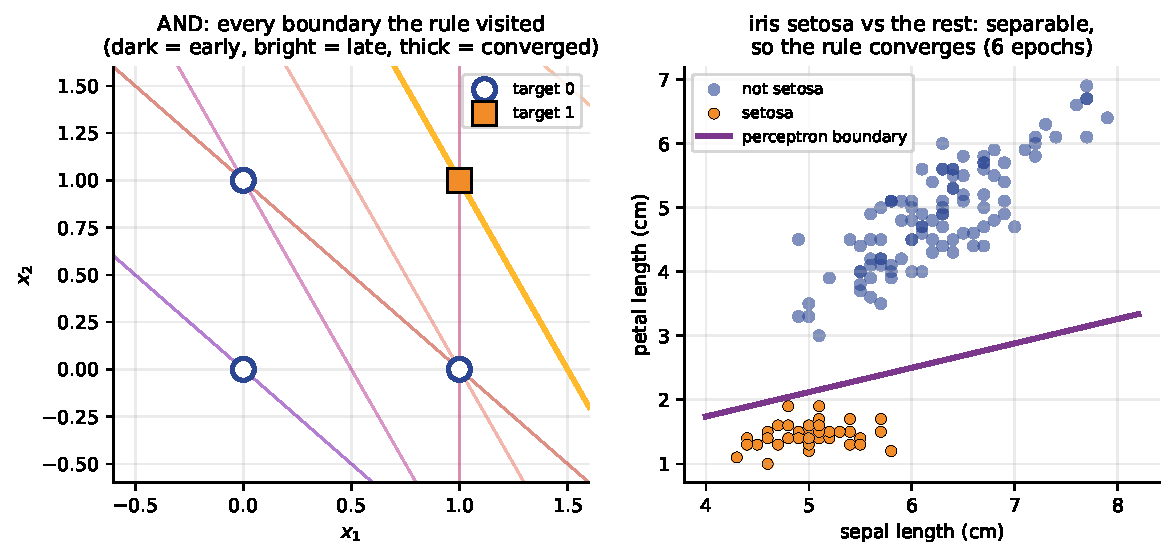
\includegraphics[width=\textwidth]{perceptron.pdf}
      \vspace{0.2em}
      {\scriptsize Left: the twelve weight states on AND, dark early, bright
      late; the thick orange line is the converged rule. Right: the same rule
      on \texttt{load\_iris}, setosa against the other two --- separable, so
      it converges, in six epochs again.\par}
    \end{column}
  \end{columns}
\end{frame}

\begin{frame}[fragile,shrink=6]{The same thing in code, on a real dataset}
\begin{lstlisting}
def perceptron_fit(X, y, epochs=100, eta=1.0):
    w, b = np.zeros(X.shape[1]), 0.0
    for ep in range(epochs):
        errors = 0
        for k in range(len(X)):
            yh = 1.0 if (w @ X[k] + b) >= 0 else 0.0
            err = y[k] - yh
            if err != 0:
                w, b, errors = w + eta*err*X[k], b + eta*err, errors + 1
        if errors == 0: return w, b, ep + 1
\end{lstlisting}
\begin{outblk}
iris setosa vs rest, 150 rows, 2 features
   epoch  1  updates  1  training accuracy 0.6667
   epoch  4  updates  2  training accuracy 0.6667
   epoch  5  updates  1  training accuracy 1.0000
   epoch  6  updates  0  training accuracy 1.0000
   converged in 6 epochs, final training accuracy 1.0000
   final weights w = [+3.50 -9.20]  b = +2.00
   sklearn Perceptron on the same data: accuracy 1.0000
\end{outblk}
  \begin{center}\small
    Eight lines. \texttt{sklearn.linear\_model.Perceptron} is the same rule
    with bookkeeping.
  \end{center}
\end{frame}

\begin{frame}[shrink=4]{What the rule guarantees --- and what it does not}
  \begin{columns}[T]
    \begin{column}{0.49\textwidth}
      \begin{exampleblock}{Perceptron convergence theorem}
        If the two classes are \textbf{linearly separable}, the rule reaches
        zero training errors in a finite number of updates, bounded by
        $(R/\gamma)^2$ where $R$ is the largest $\|x\|$ and $\gamma$ the
        margin of the best separator. It does not depend on $\eta$, on the
        order of the rows, or on where you start.
      \end{exampleblock}
    \end{column}
    \begin{column}{0.49\textwidth}
      \begin{alertblock}{And if they are not separable?}
        The theorem says nothing, and neither does the algorithm. It does not
        converge, it does not warn you, and it does not return the best line
        it saw. It \textbf{cycles forever}.

        \medskip
        There is no ``stop when the error stops improving'' in the rule as
        Rosenblatt stated it. That is not a small print issue --- it is the
        subject of the next section.
      \end{alertblock}
    \end{column}
  \end{columns}
\end{frame}

% =====================================================================
\section[XOR]{XOR: the wall, and the way through}
\label{sec:xor}

\begin{frame}[shrink=6]{Predict first \#2 --- exclusive OR}
  \begin{alertblock}{Commit to a number}
    Four rows again: $(0,0)\to 0$, $(0,1)\to \mathbf{1}$,
    $(1,0)\to \mathbf{1}$, $(1,1)\to 0$. Output $1$ when the inputs
    \emph{differ}.

    \medskip
    Run the perceptron rule for a thousand epochs.

    \medskip
    \centering\large
    What training accuracy does it end on?\\
    And what is the best accuracy \emph{any} straight line can get?
  \end{alertblock}
  \onslide<2->{
  \begin{exampleblock}{}
    \centering\large
    The rule ends on $\mathbf{0.50}$. The best line achieves $\mathbf{0.75}$.
  \end{exampleblock}
  \begin{center}\small
    Two separate failures. No line gets all four --- and the learning rule
    does not even find the best line, because it never stops correcting.
  \end{center}}
\end{frame}

\begin{frame}[shrink=6]{Why no line works}
  \begin{columns}[T]
    \begin{column}{0.46\textwidth}
      \begin{block}{The geometry, in one sentence}
        A line cuts the plane into two half-planes. The two $1$s sit at
        $(0,1)$ and $(1,0)$ --- \textbf{diagonally opposite corners} of the
        unit square. Any half-plane containing both must also contain the
        midpoint $(0.5, 0.5)$, and hence some of the segment joining the two
        $0$s.
      \end{block}
    \end{column}
    \begin{column}{0.51\textwidth}
      \begin{block}{The algebra, in four inequalities}
        Suppose $w_1x_1 + w_2x_2 + b \ge 0$ exactly on the $1$s:
        \[
          \begin{array}{ll}
            b < 0 & \text{from } (0,0) \to 0\\
            w_2 + b \ge 0 & \text{from } (0,1) \to 1\\
            w_1 + b \ge 0 & \text{from } (1,0) \to 1\\
            w_1 + w_2 + b < 0 & \text{from } (1,1) \to 0
          \end{array}
        \]
        Add rows 2 and 3: $w_1 + w_2 + 2b \ge 0$. Row 4 says
        $w_1 + w_2 + b < 0$, so $b > 0$. Contradiction with row 1.
      \end{block}
    \end{column}
  \end{columns}
  \begin{center}\small
    \textbf{Minsky and Papert, 1969.} This one page stopped neural-network
    funding for a decade.
  \end{center}
\end{frame}

\begin{frame}[fragile,shrink=6]{The same thing in code}
\begin{lstlisting}
w, b = np.zeros(2), 0.0
for ep in range(1000):
    for k in range(4):
        yh = 1.0 if (w @ X_xor[k] + b) >= 0 else 0.0
        w, b = w + (y_xor[k]-yh)*X_xor[k], b + (y_xor[k]-yh)
\end{lstlisting}
\begin{outblk}
perceptron on XOR, 1000 epochs
   best accuracy ever reached      0.50
   accuracy after the last epoch   0.50
   distinct (w1, w2, b) states visited: 2 -- it cycles, it does not settle
   sklearn Perceptron, 10000 iterations: accuracy 0.50
   logistic regression (also a single linear unit): accuracy 0.50
   exhaustive search over 81^3 = 531441 lines: the best any line achieves
   on XOR is 0.75 (3 of 4 rows), e.g. w = (-4.0, -4.0), b = +4.0
\end{outblk}
  \begin{center}\small
    Two end-of-epoch states, visited alternately, for a thousand epochs.
    Logistic regression --- which \emph{is} differentiable and \emph{does}
    minimise a loss --- gets $0.50$ too, because it is still one linear unit.
  \end{center}
\end{frame}

\begin{frame}[fragile,shrink=8]{By hand: two hidden units solve it}
  \begin{columns}[T]
    \begin{column}{0.44\textwidth}
      \begin{block}{Build them from what we have}
        $h_1 = \mathrm{OR}(x_1,x_2)$: weights $(1,1)$, bias $-0.5$.\\
        $h_2 = \mathrm{AND}(x_1,x_2)$: weights $(1,1)$, bias $-1.5$.\\[0.3em]
        Then $\hat y = \mathrm{OR}$ \emph{and not} $\mathrm{AND}$: weights
        $(+1, -1)$ on $(h_1, h_2)$, bias $-0.5$.
      \end{block}
    \end{column}
    \begin{column}{0.53\textwidth}
\begin{outblk}
 x1 x2 | h1=OR h2=AND | y_hat | target
  0  0  |   0     0    |   0   |   0
  0  1  |   1     0    |   1   |   1
  1  0  |   1     0    |   1   |   1
  1  1  |   1     1    |   0   |   0
accuracy 1.00
hidden representation of the four inputs:
   (0,0) -> (0,0)
   (0,1) -> (1,0)
   (1,0) -> (1,0)
   (1,1) -> (1,1)
\end{outblk}
    \end{column}
  \end{columns}
  \vspace{0.2em}
  \begin{center}\small
    Every one of these three units is a perceptron. Nothing new was invented
    --- they were only \textbf{stacked}.
  \end{center}
\end{frame}

\begin{frame}[shrink=4]{The hidden layer is a change of coordinates}
  \begin{exampleblock}{}
    \centering\large
    $(0,1)$ and $(1,0)$ both land on $(1,0)$.
  \end{exampleblock}
  \begin{columns}[T]
    \begin{column}{0.49\textwidth}
      \begin{block}{What that buys}
        In the input plane the two positives are diagonally opposite. In the
        hidden plane they are \textbf{the same point}. Three distinct points
        remain: $(0,0)$, $(1,0)$, $(1,1)$ --- and the middle one is the only
        positive. One line separates it from the other two.
      \end{block}
    \end{column}
    \begin{column}{0.49\textwidth}
      \begin{alertblock}{The general statement}
        A hidden layer does not classify. It \textbf{re-represents}: it maps
        the input into a new space chosen so that the last layer's linear
        model works there. Everything a deep network does is this, repeated.

        \medskip
        The output layer is always just logistic (or linear) regression. The
        layers below it are learning the features that regression needed.
      \end{alertblock}
    \end{column}
  \end{columns}
\end{frame}

\begin{frame}[shrink=10]{Drawn: XOR, before and after the hidden layer}
  \begin{center}
    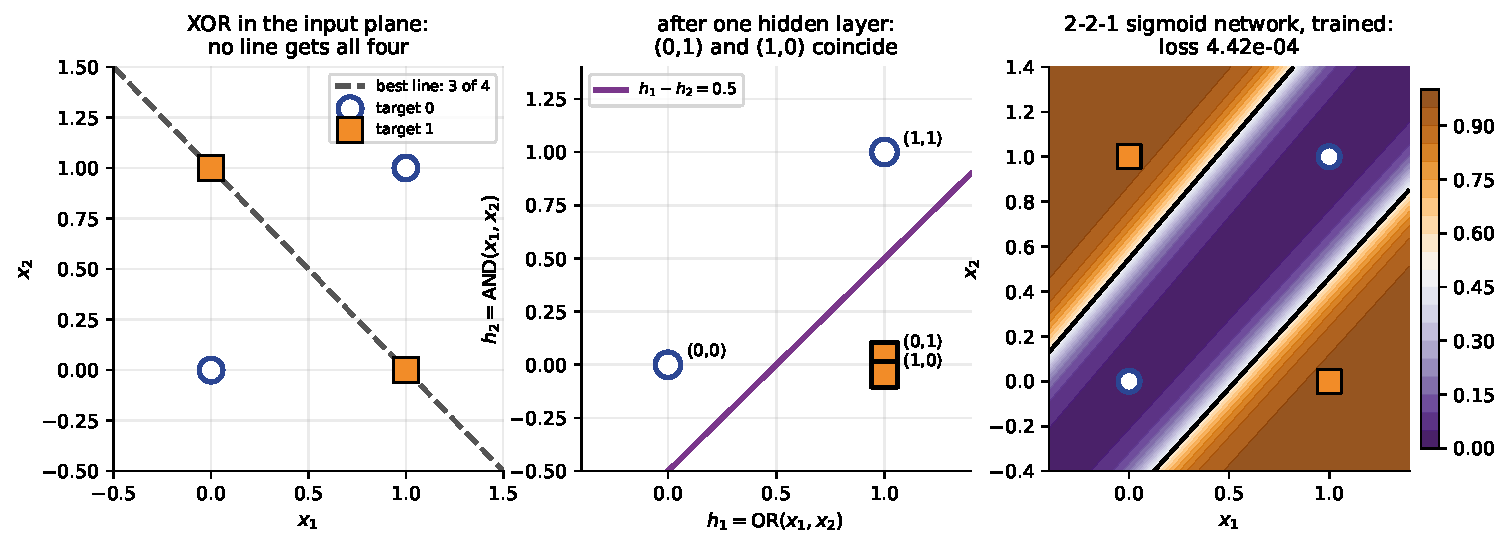
\includegraphics[width=0.86\textwidth]{xor.pdf}
  \end{center}
  \begin{center}\small
    Left: the best line, three of four. Middle: after the hidden layer, the
    two positives coincide and a line does exist. Right: the decision surface
    of a trained $2$--$2$--$1$ sigmoid network, final loss
    $\mathbf{3.30\times10^{-4}}$.
  \end{center}
\end{frame}

\begin{frame}[fragile,shrink=8]{And the network finds those units for itself}
\begin{outblk}
2-2-1 sigmoid network trained on XOR, 20000 steps of full-batch descent
   loss at step     0: 0.125700
   loss at step  1000: 0.125008
   loss at step 20000: 0.000442
   outputs [0.0299 0.9717 0.9663 0.0265] against targets [0 1 1 0]
   accuracy 1.00
   learned hidden weights
      unit 1: w = [-5.80 +5.91]  b = +2.96
      unit 2: w = [-5.37 +5.17]  b = -2.81
   output layer: w = [-8.17 +8.66]  b = +3.80
   hidden units 1 -> final loss 0.118611
   hidden units 2 -> final loss 0.000442
\end{outblk}
  \begin{center}\small
    It did \emph{not} learn OR and AND. Unit 2 fires on
    ``$x_2$ and not $x_1$''; unit 1 fires everywhere \emph{except} $(1,0)$
    and the output weight on it is $-8.17$, so what reaches the output is
    ``$x_1$ and not $x_2$'' upside down. Same decomposition, one half
    inverted --- and with \textbf{one} hidden unit the loss stalls at
    $0.1186$, barely below its starting $0.1257$.
  \end{center}
\end{frame}

\begin{frame}[shrink=6]{The feedforward network, in general}
  \begin{exampleblock}{}
    \centering\large
    $a^{(0)} = x$, \qquad
    $z^{(\ell)} = W^{(\ell)\top} a^{(\ell-1)} + b^{(\ell)}$, \qquad
    $a^{(\ell)} = \varphi^{(\ell)}\!\left(z^{(\ell)}\right)$
  \end{exampleblock}
  \begin{columns}[T]
    \begin{column}{0.49\textwidth}
      \begin{block}{The vocabulary the exam uses}
        \textbf{Feedforward} --- the graph has no cycles; information moves
        input to output, once.\\[0.2em]
        \textbf{Fully connected / dense} --- every unit in layer $\ell$ reads
        every unit in $\ell-1$.\\[0.2em]
        \textbf{Multi-layer perceptron (MLP)} --- a feedforward, fully
        connected network with at least one hidden layer and a
        \emph{differentiable} activation.
      \end{block}
    \end{column}
    \begin{column}{0.49\textwidth}
      \begin{alertblock}{An MLP is not made of perceptrons}
        The name is historical and misleading. A perceptron has a step
        activation; an MLP must not, because backpropagation needs a
        derivative. Say ``unit'' or ``neuron'', not ``perceptron'', when you
        describe a hidden layer.
      \end{alertblock}
      \begin{block}{Counting parameters}
        A $64$--$32$--$10$ network has
        $64{\cdot}32 + 32 + 32{\cdot}10 + 10 = \mathbf{2410}$.
      \end{block}
    \end{column}
  \end{columns}
\end{frame}

% =====================================================================
\section[Activations]{Activation functions, and why they are not optional}
\label{sec:act}

\begin{frame}[shrink=4]{Take the activation away and the network collapses}
  \begin{block}{Three linear layers}
    \[
      f(x) = \big((x W_1 + b_1)W_2 + b_2\big)W_3 + b_3
           = x\,\underbrace{W_1W_2W_3}_{W_{\text{eff}}}
             + \underbrace{b_1W_2W_3 + b_2W_3 + b_3}_{b_{\text{eff}}}
    \]
  \end{block}
  \begin{columns}[T]
    \begin{column}{0.49\textwidth}
      \begin{exampleblock}{The proof is one line of algebra}
        A product of matrices is a matrix. A composition of affine maps is an
        affine map. \textbf{Depth without non-linearity buys nothing at all.}
      \end{exampleblock}
    \end{column}
    \begin{column}{0.49\textwidth}
      \begin{alertblock}{And the rank bound is worse}
        $W_{\text{eff}} = W_1W_2W_3$ is $4 \times 2$, so its rank is at most
        $\min(4,6,5,2) = 2$. A narrow middle layer \emph{caps} what the whole
        stack can express, however wide the rest is.
      \end{alertblock}
    \end{column}
  \end{columns}
\end{frame}

\begin{frame}[fragile,shrink=5]{The same thing in code, then on real data}
\begin{lstlisting}
deep  = ((X @ W1 + b1) @ W2 + b2) @ W3 + b3
W_eff = W1 @ W2 @ W3
b_eff = b1 @ W2 @ W3 + b2 @ W3 + b3
flat  = X @ W_eff + b_eff
print(np.abs(deep - flat).max())
\end{lstlisting}
\begin{outblk}
three linear layers 4->6->5->2, no activation
   parameters in the deep version : 77
   parameters in the flat version : 10
   max |deep(x) - flat(x)| over 7 inputs: 7.105e-15
   W_eff = W1 W2 W3 has shape (4, 2) and rank 2
moons, 400 points
   logistic regression (1 linear unit)      accuracy 0.8750
   MLP 32-32 with identity activation       accuracy 0.8775
   MLP 32-32 with relu activation           accuracy 0.9625
   1058 parameters bought the identity network +0.0025 over 3 parameters
\end{outblk}
  \begin{center}\small
    $7.1\times10^{-15}$ is floating-point noise: the two functions are the
    same function. And $1058$ identity-activated parameters beat $3$ by
    $0.0025$ --- which is one point out of four hundred.
  \end{center}
\end{frame}

\begin{frame}[shrink=10]{Drawn: what the activation is worth}
  \begin{center}
    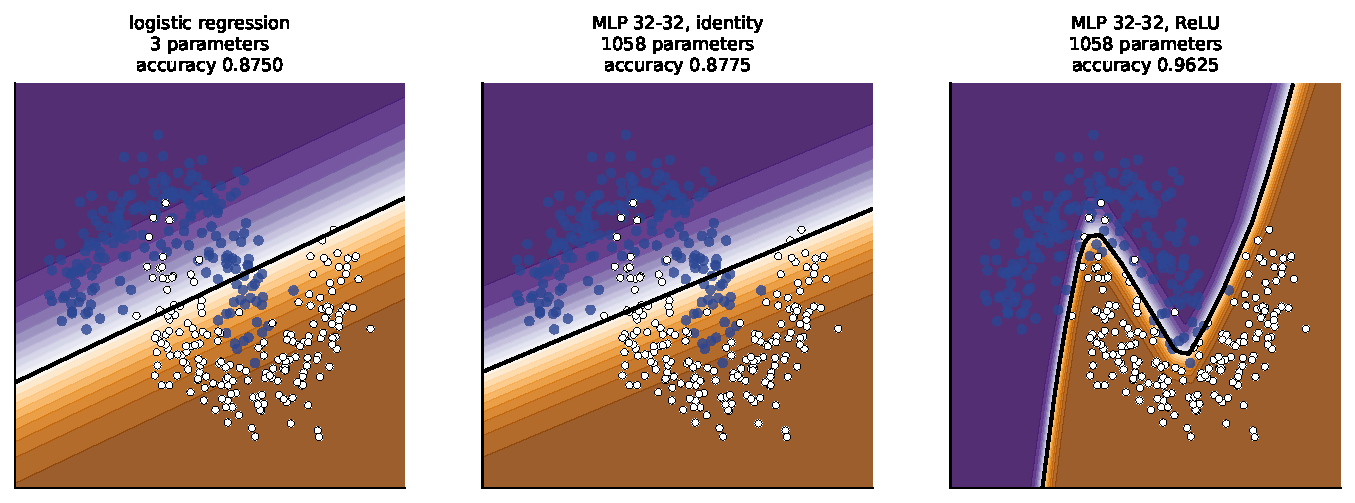
\includegraphics[width=0.84\textwidth]{linear.pdf}
  \end{center}
  \begin{center}\small
    Same architecture, same data, same optimiser. The middle panel has $1058$
    parameters and draws a straight line, because that is all it can draw.
    Swap \texttt{identity} for \texttt{relu} and the boundary bends.
  \end{center}
\end{frame}

\begin{frame}[fragile,shrink=8]{The three activations, and the derivatives backprop needs}
  \begin{columns}[T]
    \begin{column}{0.44\textwidth}
      \begin{block}{Definitions and derivatives}
        \small
        $\sigma(z) = \dfrac{1}{1+e^{-z}}$, \quad
        $\sigma'(z) = \sigma(z)\big(1-\sigma(z)\big)$\\[0.4em]
        $\tanh z$, \quad $\tanh' z = 1 - \tanh^2 z$\\[0.4em]
        $\mathrm{ReLU}(z) = \max(0,z)$, \quad
        $\mathrm{ReLU}'(z) = \mathbf{1}[z>0]$
      \end{block}
      \begin{alertblock}{}
        \small
        Note what the first two have in common: the derivative is expressible
        \textbf{in the output}. Backprop saves $a$, never $z$.
      \end{alertblock}
    \end{column}
    \begin{column}{0.53\textwidth}
\begin{outblk}
   z      sigmoid  s'(z)     tanh    t'(z)    relu   r'(z)
 -3.0    0.0474  0.0452  -0.9951  0.0099     0.0      0
 -1.0    0.2689  0.1966  -0.7616  0.4200     0.0      0
 +0.0    0.5000  0.2500  +0.0000  1.0000     0.0      0
 +1.0    0.7311  0.1966  +0.7616  0.4200     1.0      1
 +3.0    0.9526  0.0452  +0.9951  0.0099     3.0      1
max of sigmoid'  0.250000 at z = +0.0000
max of tanh'     1.000000 at z = +0.0000
sigmoid'(z) < 0.01 whenever |z| > 4.5849
\end{outblk}
    \end{column}
  \end{columns}
  \vspace{0.2em}
  \begin{center}\small
    $\sigma'$ never exceeds $\mathbf{0.25}$. $\tanh'$ never exceeds
    $\mathbf{1}$. $\mathrm{ReLU}'$ is $\mathbf{1}$ or $\mathbf{0}$ --- a gate,
    not a scale.
  \end{center}
\end{frame}

\begin{frame}[shrink=10]{Drawn: the functions, and the panel backprop multiplies}
  \begin{center}
    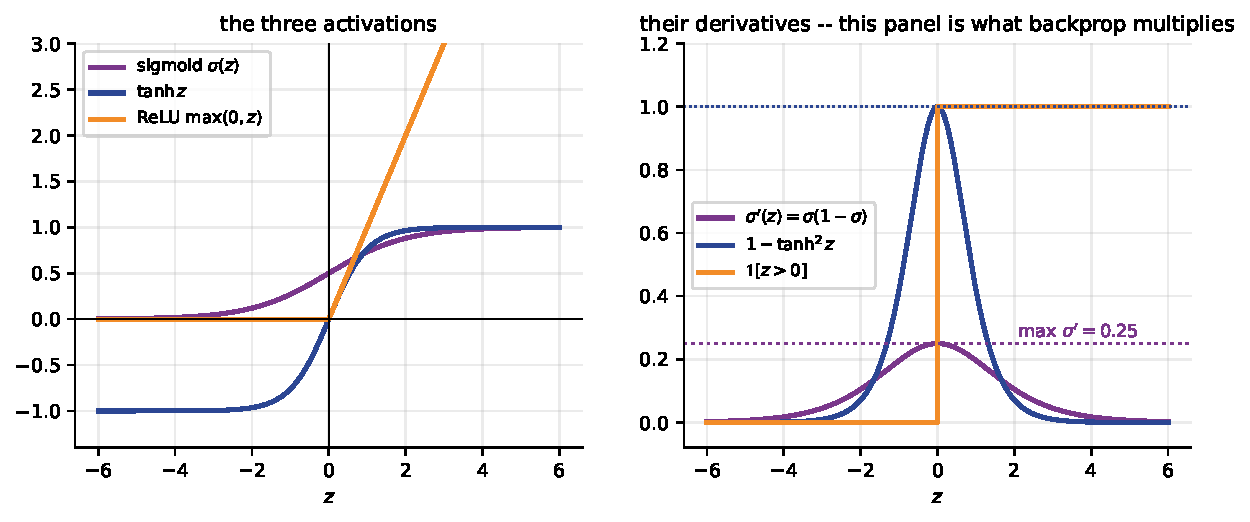
\includegraphics[width=0.74\textwidth]{activations.pdf}
  \end{center}
  \begin{center}\small
    The left panel is what the forward pass computes. \textbf{The right panel
    is what the backward pass multiplies by}, once per layer. Read the dotted
    line at $0.25$ and then look at the next slide's question.
  \end{center}
\end{frame}

\begin{frame}{Predict first \#3 --- ten sigmoid layers}
  \begin{alertblock}{Commit to an order of magnitude}
    Ten layers, sixteen units wide, \textbf{identical weights} in both
    networks. One stack uses sigmoid, the other ReLU. Push the same batch
    through, take the same loss, and measure
    $\|\partial L / \partial W^{(1)}\|$ --- the gradient reaching the layer
    nearest the input.

    \medskip
    \centering\large
    What is the ratio, ReLU over sigmoid?
  \end{alertblock}
  \onslide<2->{
  \begin{exampleblock}{}
    \centering\large
    $1.9017\times10^{-2}$ against $6.9609\times10^{-7}$:
    a factor of $\mathbf{27\,320}$.
  \end{exampleblock}
  \begin{center}\small
    And it is not a mystery. $0.25^{10} = 9.54\times10^{-7}$; the measured
    attenuation from layer 10 down to layer 1 was
    $\mathbf{8.32\times10^{-7}}$. The arithmetic predicted it.
  \end{center}}
\end{frame}

\begin{frame}[fragile,shrink=8]{The measurement, layer by layer}
\begin{outblk}
ten layers of width 16, identical weights, only the activation differs
  layer   ||dL/dW|| sigmoid   ||dL/dW|| relu      ratio relu/sigmoid
    1        6.9609e-07         1.9017e-02           27320.0
    2        4.5222e-06         2.4150e-02            5340.4
    3        1.8296e-05         1.8996e-02            1038.2
    5        3.3209e-04         1.4784e-02              44.5
    8        3.7576e-02         2.1301e-02               0.6
   10        8.3697e-01         2.8907e-02               0.0
attenuation across the sigmoid stack, layer 10 -> layer 1: 8.3167e-07
attenuation across the relu    stack, layer 10 -> layer 1: 6.5787e-01
for comparison, 0.25**9 = 3.8147e-06 and 0.25**10 = 9.5367e-07
\end{outblk}
  \begin{center}\small
    Read the sigmoid column upwards: it falls by roughly a factor of three to
    six \textbf{per layer}, compounding. The ReLU column is flat --- it
    ends at $0.658$ of where it started, not $10^{-7}$. At layer 10 the
    sigmoid gradient is nearly thirty times the \emph{larger} of the two;
    the damage is entirely in the propagation.
  \end{center}
\end{frame}

\begin{frame}[fragile,shrink=18]{Drawn: depth against the surviving gradient}
  \begin{center}
    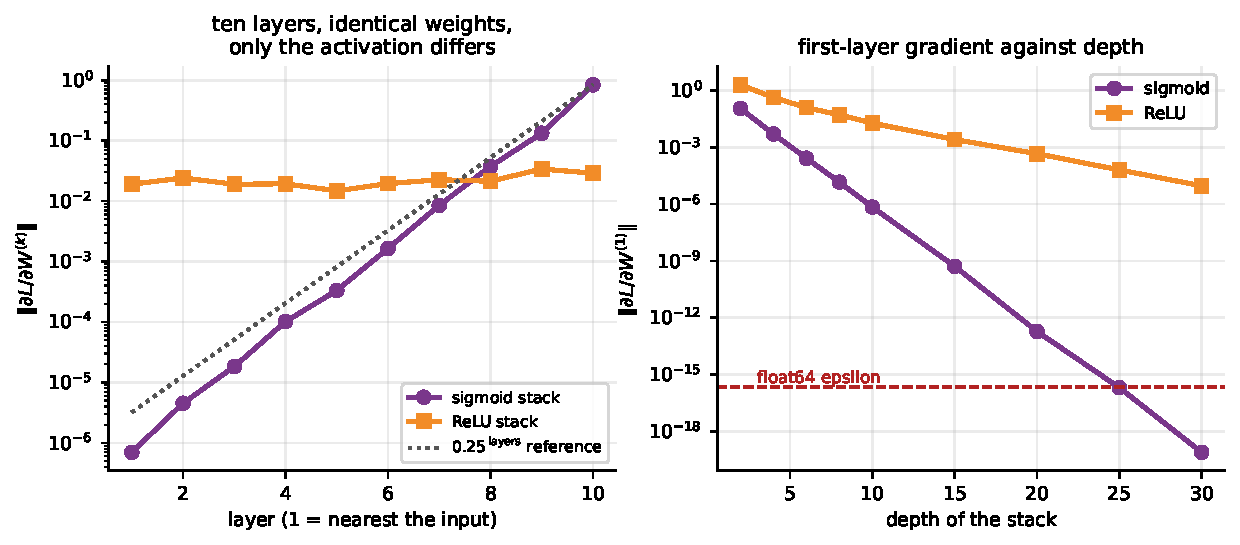
\includegraphics[width=0.72\textwidth]{vanishing.pdf}
  \end{center}
\begin{outblk}
   depth  2  sigmoid layer-1 norm 1.129e-01   relu layer-1 norm 2.009e+00
   depth 10  sigmoid layer-1 norm 6.961e-07   relu layer-1 norm 1.902e-02
   depth 30  sigmoid layer-1 norm 7.569e-20   relu layer-1 norm 9.209e-06
\end{outblk}
  \begin{center}\small
    A straight line on a log axis is geometric decay. Thirty sigmoid layers
    put the first-layer gradient at $10^{-20}$ --- far below anything single
    precision can represent against a weight of order one.
  \end{center}
\end{frame}

\begin{frame}[fragile,shrink=6]{And this is not a thought experiment}
\begin{outblk}
30 epochs, learning rate 0.1, hidden layers of 32 units each, load_digits
  activation  hidden layers   train loss   test accuracy
   relu            1           0.0758        0.9711
   relu            3           0.0114        0.9733
   relu            6           0.0030        0.9667
   relu           10           0.2811        0.8778
   sigmoid         1           0.3303        0.9422
   sigmoid         3           2.3062        0.1000
   sigmoid         6           2.3227        0.1000
   sigmoid        10           2.3184        0.1000
\end{outblk}
  \begin{center}\small
    Chance on ten balanced classes is $0.1000$, and a loss of
    $\ln 10 = 2.3026$ is the loss of a network that outputs a uniform
    distribution. \textbf{Three sigmoid hidden layers do not train at all
    here} --- not badly, at all. ReLU is fine to six layers and starts to
    strain at ten, which is an honest result and the reason residual
    connections were invented.
  \end{center}
\end{frame}

% =====================================================================
\section[Backpropagation]{Backpropagation, derived in full}
\label{sec:bp}

\begin{frame}[shrink=4]{Backpropagation is the chain rule, and nothing else}
  \begin{exampleblock}{}
    \centering\large
    $\dfrac{\partial L}{\partial x}
      = \dfrac{\partial L}{\partial y}\cdot\dfrac{\partial y}{\partial x}$
  \end{exampleblock}
  \begin{columns}[T]
    \begin{column}{0.49\textwidth}
      \begin{block}{Read the product from the left}
        For $x \to h_1 \to h_2 \to y \to L$,
        \[
          \frac{\partial L}{\partial x}
          = \frac{\partial L}{\partial y}
            \frac{\partial y}{\partial h_2}
            \frac{\partial h_2}{\partial h_1}
            \frac{\partial h_1}{\partial x}.
        \]
        Evaluate it \textbf{right to left} and you need one pass per input:
        a million parameters, a million passes. Evaluate it
        \textbf{left to right}, starting from the single number $L$, and one
        pass covers all of them.
      \end{block}
    \end{column}
    \begin{column}{0.49\textwidth}
      \begin{alertblock}{Each layer's job is local}
        A layer is handed $\partial L/\partial(\text{its output})$ and must
        return $\partial L/\partial(\text{its input})$ and
        $\partial L/\partial(\text{its parameters})$. It supplies only its
        \textbf{own} derivative and multiplies through.

        \medskip
        It does not know what is above it or below it. That locality is why
        you can write a layer once, test it once, and compose it forever.
      \end{alertblock}
    \end{column}
  \end{columns}
\end{frame}

\begin{frame}[shrink=6]{The network we are going to differentiate}
  \begin{columns}[T]
    \begin{column}{0.48\textwidth}
      \begin{block}{Two inputs, two hidden, one output}
        \small
        $x_1 = 1.0$, \; $x_2 = 2.0$, \; target $t = 1.0$\\[0.4em]
        $z_1 = w_{11}x_1 + w_{21}x_2 + b_{11}$, \; $a_1 = \sigma(z_1)$\\
        $z_2 = w_{12}x_1 + w_{22}x_2 + b_{12}$, \; $a_2 = \sigma(z_2)$\\
        $z_3 = v_1a_1 + v_2a_2 + b_2$, \; $a_3 = \sigma(z_3)$\\[0.4em]
        $L = \tfrac{1}{2}(a_3 - t)^2$
      \end{block}
    \end{column}
    \begin{column}{0.48\textwidth}
      \begin{exampleblock}{The nine parameters}
        \small
        \begin{tabular}{llll}
          \toprule
          $w_{11}$ & $+0.2$ & $w_{12}$ & $+0.3$\\
          $w_{21}$ & $-0.1$ & $w_{22}$ & $+0.1$\\
          $b_{11}$ & $\phantom{+}0.0$ & $b_{12}$ & $+0.5$\\
          $v_1$ & $+0.4$ & $v_2$ & $-0.6$\\
          $b_2$ & $+0.1$ & &\\
          \bottomrule
        \end{tabular}
      \end{exampleblock}
    \end{column}
  \end{columns}
  \vspace{0.2em}
  \begin{center}\small
    Nine parameters is small enough to do entirely with a pen and large
    enough that every case appears: two layers, a shared downstream path, and
    biases. \textbf{Copy these numbers down.}
  \end{center}
\end{frame}

\begin{frame}[fragile,shrink=8]{Forward pass, by hand}
  \begin{block}{}
    \small
    \begin{align*}
      z_1 &= (0.2)(1.0) + (-0.1)(2.0) + 0.0 = 0.0
            &&a_1 = \sigma(0) = \mathbf{0.5000000000}\\
      z_2 &= (0.3)(1.0) + (0.1)(2.0) + 0.5 = 1.0
            &&a_2 = \sigma(1) = \mathbf{0.7310585786}\\
      z_3 &= (0.4)(0.5) + (-0.6)(0.7310585786) + 0.1 = \mathbf{-0.1386351472}
            &&a_3 = \sigma(z_3) = \mathbf{0.4653966177}
    \end{align*}
    \[
      L = \tfrac12(0.4653966177 - 1)^2 = \tfrac12(-0.5346033823)^2
        = \mathbf{0.1429003882}
    \]
  \end{block}
\begin{outblk}
z1 = 0.2*1.0 + -0.1*2.0 + 0.0 = +0.0000   a1 = sigma(z1) = 0.5000000000
z2 = 0.3*1.0 + 0.1*2.0 + 0.5 = +1.0000   a2 = sigma(z2) = 0.7310585786
z3 = 0.4*0.5000000000 + -0.6*0.7310585786 + 0.1 = -0.1386351472
a3 = sigma(z3) = 0.4653966177
L  = 0.5 * (0.4653966177 - 1.0)^2 = 0.1429003882
\end{outblk}
  \begin{center}\small
    The two weights were chosen so $z_1 = 0$ exactly: $\sigma(0) = 0.5$ and
    $\sigma'(0) = 0.25$, both by hand.
  \end{center}
\end{frame}

\begin{frame}[shrink=10]{Drawn: the same network, forward and backward}
  \begin{center}
    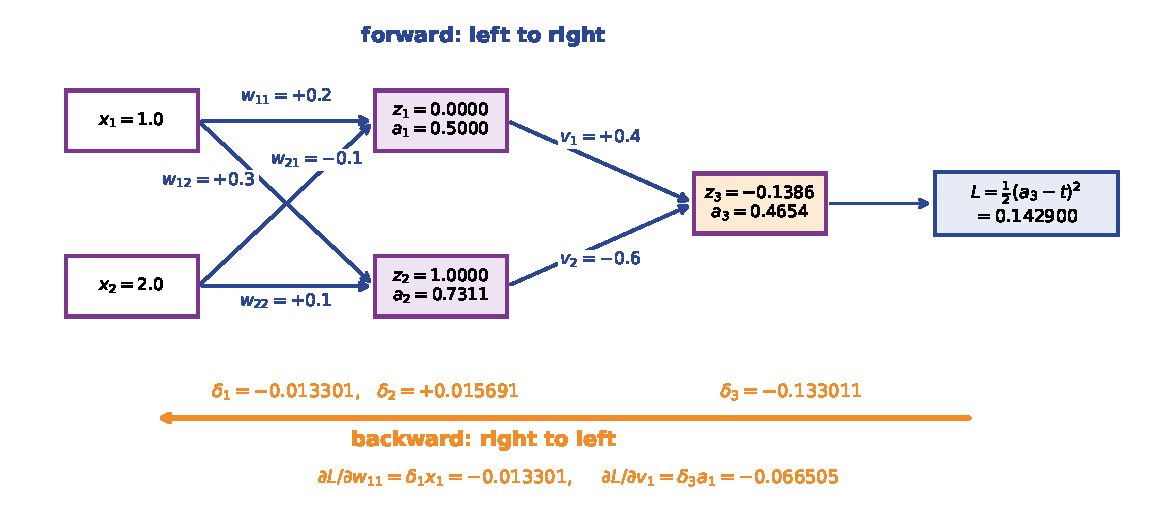
\includegraphics[width=0.80\textwidth]{tinynet.pdf}
  \end{center}
  \begin{center}\small
    Every number on this figure was produced by the code, not typed onto it.
    The orange arrow is the direction of the next four slides.
  \end{center}
\end{frame}

\begin{frame}[shrink=5]{Backward, step 1: the output unit}
  \begin{block}{Two factors, then their product}
    \begin{align*}
      \frac{\partial L}{\partial a_3}
        &= a_3 - t = 0.4653966177 - 1 = \mathbf{-0.5346033823}\\[0.3em]
      \frac{\partial a_3}{\partial z_3}
        &= a_3(1 - a_3) = (0.4653966177)(0.5346033823)
         = \mathbf{+0.2488026059}\\[0.3em]
      \delta_3 \;\equiv\; \frac{\partial L}{\partial z_3}
        &= \frac{\partial L}{\partial a_3}\cdot\frac{\partial a_3}{\partial z_3}
         = (-0.5346033823)(0.2488026059) = \mathbf{-0.1330107147}
    \end{align*}
  \end{block}
  \begin{center}\small
    $\delta_3$ is the whole of the output layer's message to everything
    below. \textbf{One number}. Every gradient in the network is $\delta_3$
    multiplied by something local.
  \end{center}
\end{frame}

\begin{frame}[shrink=6]{Backward, step 2: the output layer's own weights}
  \begin{block}{Because $z_3 = v_1a_1 + v_2a_2 + b_2$}
    \begin{align*}
      \frac{\partial L}{\partial v_1}
        &= \delta_3 \cdot \frac{\partial z_3}{\partial v_1} = \delta_3 a_1
         = (-0.1330107147)(0.5000000000) = \mathbf{-0.0665053573}\\
      \frac{\partial L}{\partial v_2}
        &= \delta_3 a_2
         = (-0.1330107147)(0.7310585786) = \mathbf{-0.0972386240}\\
      \frac{\partial L}{\partial b_2}
        &= \delta_3 \cdot 1 = \mathbf{-0.1330107147}
    \end{align*}
  \end{block}
  \begin{columns}[T]
    \begin{column}{0.55\textwidth}
      \begin{exampleblock}{The pattern, already visible}
        \centering
        gradient of a weight $=$ \textbf{delta} $\times$ \textbf{the
        activation it multiplies}
      \end{exampleblock}
    \end{column}
    \begin{column}{0.42\textwidth}
      \begin{alertblock}{}
        \small A bias multiplies the constant $1$, so its gradient is the
        delta itself. That is the whole rule for biases.
      \end{alertblock}
    \end{column}
  \end{columns}
\end{frame}

\begin{frame}[shrink=6]{Backward, step 3: push the delta through the hidden layer}
  \begin{block}{The recursion --- this is the line that makes it
    ``back''-propagation}
    \begin{align*}
      \delta_1 \;\equiv\; \frac{\partial L}{\partial z_1}
        &= \underbrace{\delta_3}_{\text{from above}}
           \cdot \underbrace{v_1}_{\text{the path}}
           \cdot \underbrace{a_1(1-a_1)}_{\sigma'(z_1)}
         = (-0.1330107147)(0.4)(0.25) = \mathbf{-0.0133010715}\\
      \delta_2 \;\equiv\; \frac{\partial L}{\partial z_2}
        &= \delta_3 \cdot v_2 \cdot a_2(1-a_2)\\
        &= (-0.1330107147)(-0.6)(0.7310585786)(0.2689414214)
         = \mathbf{+0.0156908963}
    \end{align*}
  \end{block}
  \begin{center}\small
    Three things happened to the message: it was \textbf{routed} along the
    weight it came down ($v_j$), and \textbf{throttled} by the local
    derivative ($\sigma'$). Note $\delta_2$ has the \emph{opposite sign} to
    $\delta_3$, because $v_2$ is negative. And
    $a_1(1-a_1) = 0.25$ exactly: this unit sits at the steepest point of the
    sigmoid, the most gradient it can ever pass.
  \end{center}
\end{frame}

\begin{frame}[shrink=6]{Backward, step 4: the input layer's weights}
  \begin{block}{Same rule as step 2, one layer down: delta $\times$ input}
    \begin{align*}
      \frac{\partial L}{\partial w_{11}} &= \delta_1 x_1
        = (-0.0133010715)(1.0) = \mathbf{-0.0133010715}\\
      \frac{\partial L}{\partial w_{21}} &= \delta_1 x_2
        = (-0.0133010715)(2.0) = \mathbf{-0.0266021429}\\
      \frac{\partial L}{\partial b_{11}} &= \delta_1
        = \mathbf{-0.0133010715}\\
      \frac{\partial L}{\partial w_{12}} &= \delta_2 x_1
        = \mathbf{+0.0156908963}\\
      \frac{\partial L}{\partial w_{22}} &= \delta_2 x_2
        = \mathbf{+0.0313817925}\\
      \frac{\partial L}{\partial b_{12}} &= \delta_2
        = \mathbf{+0.0156908963}
    \end{align*}
  \end{block}
  \begin{center}\small
    $\partial L/\partial w_{21}$ is exactly twice
    $\partial L/\partial w_{11}$ because $x_2 = 2x_1$. \textbf{An input twice
    as large gets a gradient twice as large} --- which is why you scale your
    features before training a network.
  \end{center}
\end{frame}

\begin{frame}[shrink=6]{The two rules, stated once, for any depth}
  \begin{exampleblock}{}
    \centering\large
    $\delta^{(\ell)} = \left(W^{(\ell+1)}\delta^{(\ell+1)}\right)
      \odot \varphi'\!\left(z^{(\ell)}\right)$
    \qquad\qquad
    $\dfrac{\partial L}{\partial W^{(\ell)}} = a^{(\ell-1)}\delta^{(\ell)\top}$
  \end{exampleblock}
  \begin{columns}[T]
    \begin{column}{0.49\textwidth}
      \begin{block}{That is the entire algorithm}
        Start at the top with
        $\delta^{(L)} = \nabla_{a}L \odot \varphi'(z^{(L)})$. Apply the left
        rule to walk down. Apply the right rule at each layer to read off the
        gradients. Add $\partial L/\partial b^{(\ell)} = \delta^{(\ell)}$
        and you are finished.
      \end{block}
    \end{column}
    \begin{column}{0.49\textwidth}
      \begin{alertblock}{Two shapes to get right}
        The $\odot$ is \textbf{elementwise}: the activation derivative is a
        diagonal Jacobian, so it never becomes a matrix product. And for a
        batch of $n$ rows, the bias gradient is the \textbf{sum over the
        batch}, because one bias was copied $n$ times. That summation is the
        single commonest bug in a hand-written backward pass.
      \end{alertblock}
    \end{column}
  \end{columns}
\end{frame}

\begin{frame}[shrink=8]{Predict first \#4 --- is the derivation right?}
  \begin{alertblock}{Commit to an exponent}
    We now have nine numbers computed with a pen. Check them the dumb way:
    for each parameter $p$, nudge it by $h = 10^{-6}$ each way, run the
    forward pass twice, and take
    $\big(L(p{+}h) - L(p{-}h)\big) / 2h$.

    \medskip
    \centering\large
    How closely will the two agree?\\
    \normalsize (Give it as a power of ten.)
  \end{alertblock}
  \onslide<2->{
  \begin{exampleblock}{}
    \centering\large
    Largest disagreement over all nine: $\mathbf{4.107\times10^{-11}}$.
  \end{exampleblock}
  \begin{center}\small
    And that residue is the \emph{finite difference's} error, not
    backpropagation's. The central difference is accurate to $O(h^2)$, and
    with $h = 10^{-6}$ that is $O(10^{-12})$, degraded a little by
    cancellation in the subtraction.
  \end{center}}
\end{frame}

\begin{frame}[fragile,shrink=8]{Verified once: central finite differences}
\begin{lstlisting}
h = 1e-6
for k in base:                       # base = the nine parameters
    up, dn = dict(base), dict(base)
    up[k], dn[k] = base[k] + h, base[k] - h
    fd = (tiny_loss(up) - tiny_loss(dn)) / (2 * h)
    print(k, hand[k], fd, abs(fd - hand[k]))
\end{lstlisting}
\begin{outblk}
parameter   hand-computed      finite difference    |difference|
   w11      -0.013301071466     -0.013301071425     4.107e-11
   w12      +0.015690896251     +0.015690896291     4.005e-11
   w21      -0.026602142932     -0.026602142905     2.662e-11
   w22      +0.031381792501     +0.031381792540     3.846e-11
   b11      -0.013301071466     -0.013301071425     4.107e-11
   b12      +0.015690896251     +0.015690896291     4.005e-11
   v1       -0.066505357329     -0.066505357305     2.492e-11
   v2       -0.097238624001     -0.097238623986     1.502e-11
   b2       -0.133010714659     -0.133010714679     1.954e-11
largest disagreement over all nine parameters: 4.107e-11
\end{outblk}
  \begin{center}\small
    Nine for nine, to ten significant figures. \textbf{Do this every time you
    write a backward pass by hand.} A gradient that is wrong by a factor of
    two still trains, just worse, and you will blame the learning rate for a
    week.
  \end{center}
\end{frame}

\begin{frame}[fragile,shrink=9]{Verified twice: autodiff, in a library you can open}
\begin{lstlisting}
import gradkit as gk
W1g = gk.tensor(W1, requires_grad=True); b1g = gk.tensor(b1, requires_grad=True)
W2g = gk.tensor(W2.reshape(2,1), requires_grad=True); b2g = gk.tensor([b2], requires_grad=True)
a1g = gk.sigmoid(gk.tensor(x.reshape(1,2)) @ W1g + b1g)
a2g = gk.sigmoid(a1g @ W2g + b2g)
Lg  = ((a2g - tg) * (a2g - tg)).sum() * 0.5
Lg.backward()
\end{lstlisting}
\begin{outblk}
gradkit forward loss  0.142900388188   (hand: 0.142900388188)
parameter    hand            gradkit          |difference|
   w11    -0.013301071466   -0.013301071466    0.000e+00
   w21    -0.026602142932   -0.026602142932    0.000e+00
   v1     -0.066505357329   -0.066505357329    0.000e+00
   b2     -0.133010714659   -0.133010714659    0.000e+00
largest hand-vs-autodiff disagreement: 0.000e+00
largest hand-vs-finite-difference disagreement: 4.107e-11
all nine hand-computed gradients confirmed twice
\end{outblk}
  \begin{center}\small
    \textbf{Zero}, bit for bit --- because autodiff evaluates the same
    product of the same local derivatives, in the same order.
    \texttt{gradkit} is written for this course; open
    \texttt{functions/activation.py} and you will find $\sigma(1-\sigma)$
    exactly as we wrote it. \texttt{\url{https://github.com/tali7c/gradkit}}
  \end{center}
\end{frame}

\begin{frame}[fragile,shrink=6]{What you do with nine gradients}
\begin{outblk}
one step of gradient descent, p <- p - eta * dL/dp
   eta   0.5   loss 0.1429003882 -> 0.1263134462   (-1.66e-02)
   eta   5.0   loss 0.1429003882 -> 0.0297255097   (-1.13e-01)
   eta  50.0   loss 0.1429003882 -> 0.0000000004   (-1.43e-01)
   after   1 steps at eta=5.0: loss 0.02972551  output 0.756174
   after  10 steps at eta=5.0: loss 0.00262249  output 0.927578
   after 100 steps at eta=5.0: loss 0.00021488  output 0.979270
   after 500 steps at eta=5.0: loss 0.00003898  output 0.991170
\end{outblk}
  \begin{center}\small
    The output climbs $0.4654 \to 0.7562 \to 0.9912$ towards the target
    $1.0$. Do not read too much into $\eta = 50$ working here: this is
    \emph{one} training row and one row can always be fitted. On a real
    dataset that learning rate diverges immediately.
  \end{center}
\end{frame}

\begin{frame}[fragile,shrink=7]{One special case worth memorising: softmax with cross-entropy}
  \begin{block}{}
    \small
    With $p = \mathrm{softmax}(z)$ and $L = -\sum_c y_c \log p_c$, the
    softmax Jacobian $p_i(\delta_{ij} - p_j)$ and the $1/p$ from the
    logarithm cancel exactly, leaving
    \[
      \frac{\partial L}{\partial z} = p - y.
    \]
  \end{block}
\begin{outblk}
logits z          = [2.0 1.0 0.1]
softmax p         = [0.659001 0.242433 0.098566]
target one-hot y  = [0 1 0]
L = -log p_1      = 1.417030
claim: dL/dz = p - y = [+0.659001 -0.757567 +0.098566]
finite difference    = [+0.659001 -0.757567 +0.098566]
largest disagreement = 2.168e-10
\end{outblk}
  \begin{center}\small
    So the output layer of a classifier needs \textbf{no activation
    derivative at all} in code: the delta is just
    \texttt{(probs - onehot)}. That is why the NumPy network on the next
    slides starts its backward pass with one subtraction.
  \end{center}
\end{frame}

% =====================================================================
\section[Training an MLP]{An MLP, from scratch, on real data}
\label{sec:mlp}

\begin{frame}[shrink=6]{The algorithm in eight lines}
  \begin{block}{For each mini-batch}
    \small
    \begin{enumerate}
      \item $a^{(0)} \leftarrow X_{\text{batch}}$
      \item for $\ell = 1 \dots L$: \;
        $z^{(\ell)} = a^{(\ell-1)}W^{(\ell)} + b^{(\ell)}$, \;
        $a^{(\ell)} = \varphi(z^{(\ell)})$ \hfill \emph{forward}
      \item $\delta^{(L)} \leftarrow (a^{(L)} - Y)/n$
        \hfill \emph{softmax + cross-entropy}
      \item for $\ell = L \dots 1$:
      \item \quad $\nabla W^{(\ell)} = a^{(\ell-1)\top}\delta^{(\ell)}$, \;
        $\nabla b^{(\ell)} = \textstyle\sum_{\text{rows}} \delta^{(\ell)}$
        \hfill \emph{read off}
      \item \quad $\delta^{(\ell-1)} =
        \big(\delta^{(\ell)}W^{(\ell)\top}\big)\odot\varphi'(z^{(\ell-1)})$
        \hfill \emph{propagate}
      \item $W^{(\ell)} \leftarrow W^{(\ell)} - \eta\nabla W^{(\ell)}$ for
        every $\ell$ \hfill \emph{update}
      \item repeat over all batches; that is one \textbf{epoch}
    \end{enumerate}
  \end{block}
  \begin{center}\small
    Lines 5 and 6 are the two rules from four slides ago, in matrix form.
    Nothing else has been added.
  \end{center}
\end{frame}

\begin{frame}[fragile,shrink=8]{Written out in NumPy --- the whole thing}
\begin{lstlisting}
def forward(P, X):
    A, Z = [X], []
    for k, (W, b) in enumerate(P):
        z = A[-1] @ W + b; Z.append(z)
        A.append(softmax(z) if k == len(P)-1 else relu(z))
    return A, Z

def backward(P, A, Z, Y):
    n, grads = len(Y), [None] * len(P)
    d = (A[-1] - Y) / n                 # softmax + cross-entropy, combined
    for k in range(len(P)-1, -1, -1):
        grads[k] = [A[k].T @ d, d.sum(0)]
        if k > 0:
            d = (d @ P[k][0].T) * (Z[k-1] > 0)
    return grads
\end{lstlisting}
  \begin{center}\small
    Fourteen lines, no framework. \texttt{A[k].T @ d} is
    $a^{(\ell-1)\top}\delta^{(\ell)}$; \texttt{d.sum(0)} is the bias
    summation over the batch; \texttt{(Z[k-1] > 0)} is
    $\mathrm{ReLU}'$.
  \end{center}
\end{frame}

\begin{frame}[fragile,shrink=6]{Trained on \texttt{load\_digits}}
\begin{outblk}
load_digits: 1797 rows x 64 pixels, 10 classes
train 1347 rows, test 450 rows, pixels scaled to [0, 1]
architecture 64 -> 32 -> 10, ReLU, softmax + cross-entropy
parameters: 64*32 + 32 + 32*10 + 10 = 2410
 epoch   train loss   train acc   test acc
    1      0.4232       0.8716      0.8289
    5      0.1002       0.9740      0.9689
   10      0.0604       0.9844      0.9689
   20      0.0374       0.9918      0.9800
   40      0.0081       0.9993      0.9756
   60      0.0058       1.0000      0.9711
final test accuracy 0.9711
\end{outblk}
  \begin{center}\small
    Read the last two rows together. Training accuracy reaches
    $\mathbf{1.0000}$ and test accuracy \emph{falls} from its peak of
    $0.9800$ at epoch 20 to $0.9711$ at epoch 60. That is overfitting, and it
    is the argument for early stopping.
  \end{center}
\end{frame}

\begin{frame}[fragile,shrink=6]{Drawn: the loss curve, ours against the library's}
  \begin{center}
    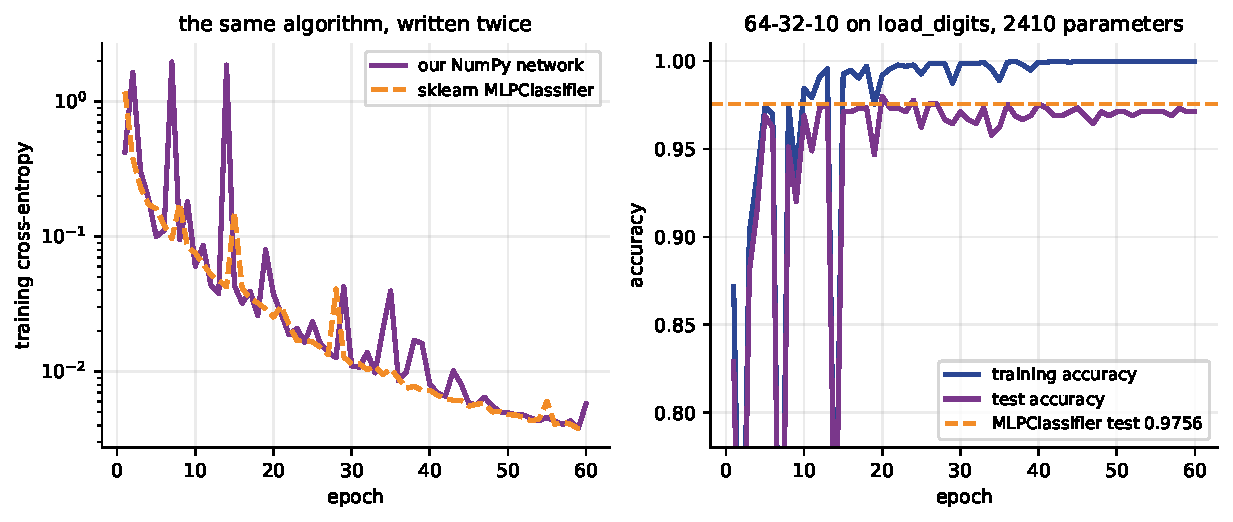
\includegraphics[width=0.84\textwidth]{losscurve.pdf}
  \end{center}
\begin{outblk}
   test accuracy from scratch, NumPy : 0.9711
   test accuracy MLPClassifier       : 0.9756   (difference +0.0044)
   MLPClassifier with its default Adam solver: 0.9733
   logistic regression, no hidden layer      : 0.9689
\end{outblk}
  \begin{center}\small
    Two independent implementations of the same fourteen lines, tracking each
    other for sixty epochs. The spikes are mini-batch noise at
    $\eta = 0.5$, present in both.
  \end{center}
\end{frame}

\begin{frame}[fragile,shrink=7]{Gradient-check the whole network, not just the toy}
\begin{outblk}
64-32-10 network, batch of 8 rows, 60 randomly chosen weight entries
layer  entry        backprop            finite difference     |diff|
  W1   (25,27)   -0.001717812303     -0.001717812292     1.02e-11
  W1   ( 5,27)   -0.046692799725     -0.046692799716     9.74e-12
  W1   ( 1,17)   -0.000164852261     -0.000164852265     3.69e-12
  W1   ( 5, 9)   -0.035753919656     -0.035753919647     9.27e-12
  W1   (29,31)   +0.036876849891     +0.036876849885     5.85e-12
largest absolute disagreement            : 2.796e-11
largest relative error where |grad|>1e-6 : 2.240e-08
\end{outblk}
  \begin{center}\small
    Many sampled entries came back \texttt{+0.000000000000} in
    \emph{both} columns. Those are border pixels that are $0$ in all eight
    rows, or dead ReLU units --- genuinely no gradient, correctly reported as
    none.
  \end{center}
\end{frame}

\begin{frame}[fragile,shrink=6]{And the same model in the course's own library}
\begin{lstlisting}
from gradkit import nn, optim
model = nn.Sequential(nn.Dense(64, 32), nn.ReLU(), nn.Dense(32, 10))
gk.fit(model, (Xtr, ytr), "cross_entropy",
       optim.SGD(model.parameters(), lr=0.5), epochs=60, batch_size=32)
\end{lstlisting}
\begin{outblk}
   test accuracy, gradkit           : 0.9667
   test accuracy, our NumPy version : 0.9711
   test accuracy, MLPClassifier     : 0.9756
three implementations of the same algorithm, three accuracies within
   0.0089 of each other.
   gradcheck(sigmoid) -> True
   gradcheck(tanh   ) -> True
   gradcheck(relu   ) -> True
\end{outblk}
  \begin{center}\small
    A spread of $0.0089$ on $450$ test rows is \textbf{four rows}. Nothing
    separates the three implementations; they are the same algorithm with
    different shuffling. Use the library to \emph{read}, not to depend on.
  \end{center}
\end{frame}

\begin{frame}{Drawn: what the hidden units actually learned}
  \begin{center}
    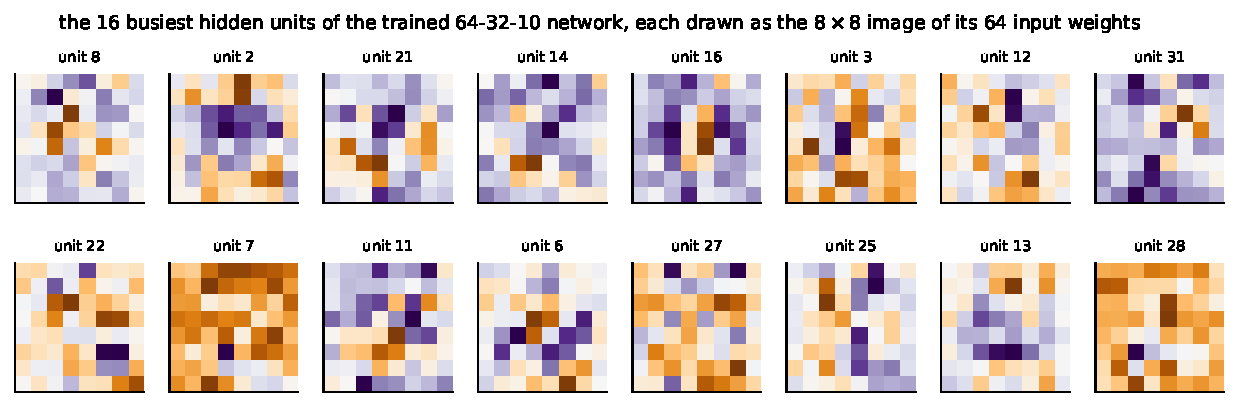
\includegraphics[width=0.94\textwidth]{hidden.pdf}
  \end{center}
  \begin{center}\small
    Each tile is one hidden unit's $64$ input weights, folded back into the
    $8\times8$ image shape. They are stroke and blob detectors --- the
    features nobody specified, discovered because the gradient said so.
  \end{center}
\end{frame}

% =====================================================================
\section[Initialisation]{Where the weights start}
\label{sec:init}

\begin{frame}{Predict first \#5 --- start everything at zero}
  \begin{alertblock}{Commit to a number}
    The same $64$--$32$--$10$ network, the same data, the same thirty epochs.
    The only change: initialise \textbf{every weight to $0$} instead of
    drawing them at random.

    \medskip
    \centering\large
    What test accuracy comes out?
  \end{alertblock}
  \onslide<2->{
  \begin{exampleblock}{}
    \centering\large
    $\mathbf{0.1000}$. Chance. Ten balanced classes, ten per cent.
  \end{exampleblock}
  \begin{center}\small
    And it is not slow learning that you could fix with more epochs. It is
    \textbf{structurally} stuck. All $32$ hidden units compute the same
    thing, receive the same gradient, and take the same step --- forever.
  \end{center}}
\end{frame}

\begin{frame}[fragile,shrink=6]{Symmetry, and why it never breaks}
  \begin{columns}[T]
    \begin{column}{0.42\textwidth}
      \begin{block}{The argument}
        If two hidden units $j$ and $k$ start with identical incoming
        weights, they compute identical $a_j = a_k$ for every input. Their
        outgoing weights are identical too, so
        $\delta_j = \delta_k$, so
        $\nabla w_{ij} = \nabla w_{ik}$, so after the update they are
        \emph{still} identical. By induction, forever.
      \end{block}
    \end{column}
    \begin{column}{0.55\textwidth}
\begin{outblk}
30 epochs, identical architecture and data
  init            train loss  train acc  test acc
  all zeros         2.3081      0.1010     0.1000
  all 0.1           2.4387      0.2517     0.2356
  He normal         0.0110      0.9985     0.9711
after training, are the 32 units distinguishable?
  zeros init : max spread across columns = 0.000e+00
  0.1   init : max spread across columns = 0.000e+00
  He    init : max spread across columns = 2.774e+00
  zeros init : columns 0 and 17 identical? True
  0.1   init : columns 0 and 17 identical? True
  He    init : columns 0 and 17 identical? False
\end{outblk}
    \end{column}
  \end{columns}
  \vspace{0.2em}
  \begin{center}\small
    It is not zero that is the problem, it is \textbf{equality}: all-$0.1$
    fails the same way and reaches $0.2356$. A $32$-unit layer with identical
    columns is a $1$-unit layer wearing a costume.
  \end{center}
\end{frame}

\begin{frame}[shrink=4]{Drawn, and the rule to use}
  \begin{center}
    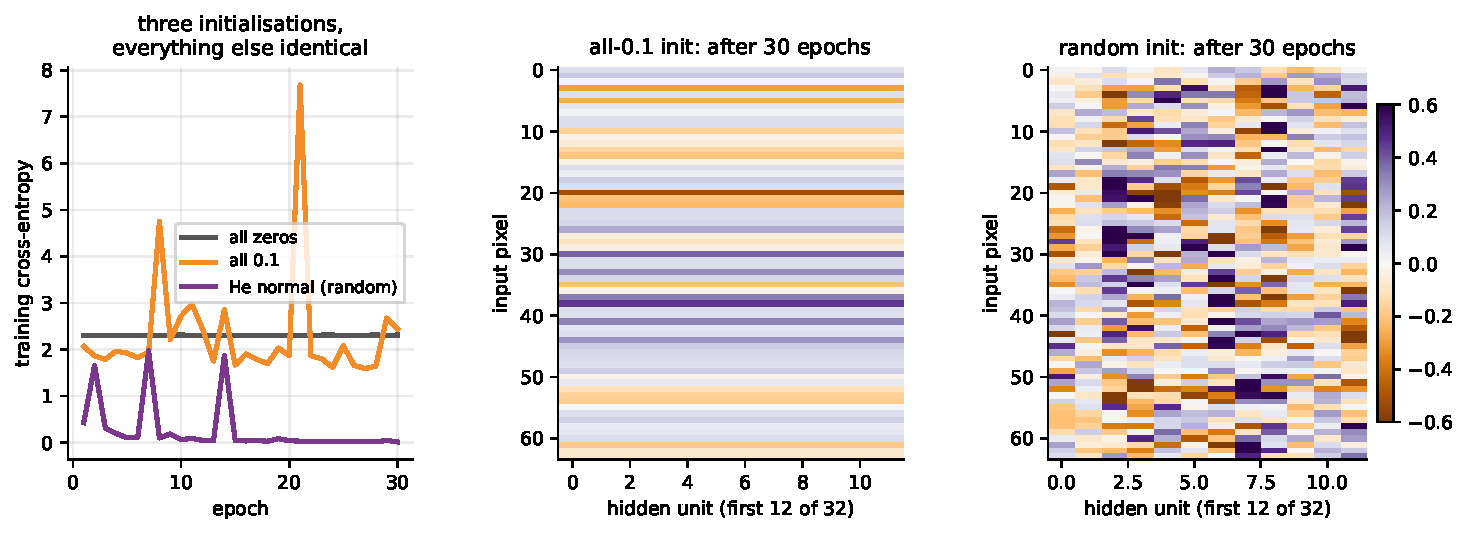
\includegraphics[width=0.92\textwidth]{init.pdf}
  \end{center}
  \begin{columns}[T]
    \begin{column}{0.49\textwidth}
      \begin{exampleblock}{}
        \centering\small
        \textbf{He}: $\mathcal{N}(0, 2/n_{\text{in}})$ for ReLU.\\
        \textbf{Xavier/Glorot}: $\mathcal{N}(0, 1/n_{\text{in}})$ for
        sigmoid and tanh.
      \end{exampleblock}
    \end{column}
    \begin{column}{0.49\textwidth}
      \begin{alertblock}{}
        \centering\small
        Biases \emph{may} start at zero --- they are not what breaks the
        symmetry, the weights are.
      \end{alertblock}
    \end{column}
  \end{columns}
\end{frame}

% =====================================================================
\section[Recurrent networks]{Recurrent and feedback architecture}
\label{sec:rnn}

\begin{frame}[shrink=5]{Add one edge that points backwards}
  \begin{exampleblock}{}
    \centering\large
    $h_t = \varphi\!\left(W_{hh}h_{t-1} + W_{xh}x_t + b\right)$, \qquad
    $y_t = W_{hy}h_t$
  \end{exampleblock}
  \begin{columns}[T]
    \begin{column}{0.49\textwidth}
      \begin{block}{What changed}
        The layer's input now includes \textbf{its own previous output}. The
        network has a state, so its answer depends on the whole history, not
        just the current input. That is what makes it suitable for
        \textbf{sequences}: text, speech, sensor streams, log files.
      \end{block}
    \end{column}
    \begin{column}{0.49\textwidth}
      \begin{alertblock}{And what did not}
        $W_{hh}$, $W_{xh}$, $W_{hy}$ and $b$ are the \textbf{same at every
        time step}. A hundred-step sequence does not have a hundred times as
        many parameters --- it reuses one small set a hundred times, exactly
        as a \texttt{for} loop reuses one body.
      \end{alertblock}
    \end{column}
  \end{columns}
  \vspace{0.2em}
  \begin{center}\small
    Also called a \textbf{feedback} architecture, against the
    \textbf{feedforward} networks of the rest of this lecture.
  \end{center}
\end{frame}

\begin{frame}[shrink=14]{Unrolling, and backpropagation through time}
  \begin{center}
    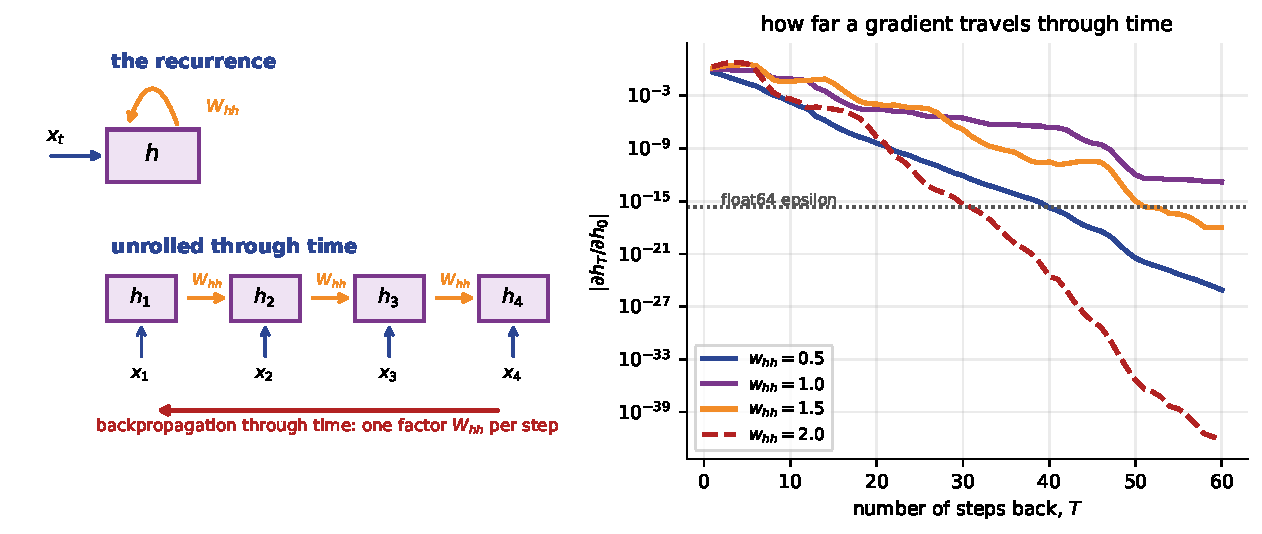
\includegraphics[width=0.78\textwidth]{rnn.pdf}
  \end{center}
  \begin{center}\small
    \textbf{Unroll} the loop over $T$ steps and you have an ordinary
    feedforward network, $T$ layers deep, whose layers share their weights.
    Backpropagation then applies unchanged --- run it on the unrolled graph
    and \emph{sum} each weight's gradient over the steps it appeared in. That
    is all \textbf{BPTT} is.
  \end{center}
\end{frame}

\begin{frame}[fragile,shrink=6]{By hand: three steps, and the gradient back to the start}
\begin{outblk}
h_t = tanh(w_hh h_{t-1} + w_xh x_t + b),   x = (1, 0, 0), w_hh = 0.9, w_xh = 1
   h1 = tanh(0.9 * 0.000000 + 1.0 * 1.0) = 0.761594
   h2 = tanh(0.9 * 0.761594 + 1.0 * 0.0) = 0.595041
   h3 = tanh(0.9 * 0.595041 + 1.0 * 0.0) = 0.489602
dh3/dh0 = prod_t w_hh (1 - h_t^2) = 0.150353
\end{outblk}
  \begin{block}{Where $0.150353$ comes from}
    \small
    $\dfrac{\partial h_T}{\partial h_0}
      = \prod_{t=1}^{T} w_{hh}\left(1 - h_t^2\right)$, and here
    $(0.9)(0.4200)\times(0.9)(0.6459)\times(0.9)(0.7603) = 0.150353$.
  \end{block}
  \begin{center}\small
    A \textbf{product of $T$ factors}. The input at $t=1$ still echoes in
    $h_3 = 0.4896$, but the gradient that would teach the network to use it
    has already shrunk to $15\%$.
  \end{center}
\end{frame}

\begin{frame}[fragile,shrink=8]{There are exactly two things that product can do}
\begin{outblk}
|dh_T/dh_0| for a scalar tanh RNN
    T     w_hh=0.5      w_hh=1.0      w_hh=1.5      w_hh=2.0
     1   4.9803e-01   9.9606e-01   1.4941e+00   1.9921e+00
     5   2.6534e-02   7.9059e-01   3.7933e+00   4.4321e+00
    10   2.0326e-04   8.5842e-02   4.2845e-02   4.4101e-04
    20   3.9998e-09   2.5262e-05   1.1633e-04   2.0875e-08
    50   3.3054e-22   1.0712e-12   1.0959e-15   4.1206e-36
   100   8.5708e-43   3.9559e-20   9.4559e-34   1.5963e-74
\end{outblk}
  \begin{center}\small
    Small factors compound to zero: the \textbf{vanishing gradient}. Large
    factors compound to infinity: the \textbf{exploding gradient} --- see
    $w_{hh} = 2.0$ more than doubling from $1.99$ to $4.43$ between $T = 1$
    and $T = 5$ before $\tanh$ saturates and drives it back down. There is no third case; $|w(1-h^2)| = 1$ exactly is
    a measure-zero accident. \textbf{Exploding is easy to fix} (clip the
    gradient norm). Vanishing is not, and that is what gates --- LSTM, GRU
    --- were invented for.
  \end{center}
\end{frame}

\begin{frame}[fragile,shrink=6]{Measured: how far back an RNN can actually remember}
\begin{outblk}
task: read a binary sequence of length T, report its FIRST symbol.
one tanh recurrent unit bank of width 8, plain BPTT, 400 epochs.
      T   held-out accuracy   ||gradient at t=1|| at epoch 0
      2       1.0000              3.335e-03
      5       1.0000              3.976e-04
     10       1.0000              2.088e-05
     20       0.5500              9.086e-08
     40       0.4925              1.527e-12
\end{outblk}
  \begin{center}\small
    The task does not get harder with $T$ --- the answer is sitting at
    $t = 1$ every time, and the other symbols are pure distraction. The
    \emph{only} thing that changes is how far the gradient has to travel. At
    $T = 40$ it arrives at $10^{-12}$ and the network scores $0.4925$: a coin.
    \textbf{This is the vanishing gradient measured on a task, not a
    diagram.}
  \end{center}
\end{frame}

% =====================================================================
\section{Summary}
\label{sec:summary}

\begin{frame}[shrink=24]{Summary --- fourteen lines}
  \begin{enumerate}\small
    \item A unit is $\varphi(w^\top x + b)$. With $\varphi = $ identity it is
      linear regression, with $\sigma$ it is logistic regression, with a step
      it is a \textbf{perceptron}.
    \item The perceptron rule $w \leftarrow w + \eta(y-\hat y)x$ is
      mistake-driven. On AND it converges in $\mathbf{6}$ epochs and
      $\mathbf{11}$ updates to $2x_1 + x_2 - 3 \ge 0$; on separable iris, $6$
      epochs to accuracy $1.0000$.
    \item If the data is not separable the rule \textbf{cycles forever}. On
      XOR it ends at $0.50$, revisiting two states; the best of all $531\,441$
      lines searched gets only $\mathbf{0.75}$.
    \item Two hidden units fix XOR by moving $(0,1)$ and $(1,0)$ to the same
      point. A hidden layer \textbf{re-represents}; the output layer is still
      just linear.
    \item Without a non-linearity, depth is free of charge and worth nothing:
      three layers with $77$ parameters equal one with $10$ to
      $\mathbf{7.1\times10^{-15}}$, and on moons, $1058$ identity parameters
      beat $3$ by $0.0025$ against ReLU's $+0.0875$.
    \item $\sigma' \le \mathbf{0.25}$, $\tanh' \le 1$, $\mathrm{ReLU}' \in
      \{0,1\}$. Ten sigmoid layers attenuate the first-layer gradient to
      $\mathbf{6.96\times10^{-7}}$ against ReLU's $1.90\times10^{-2}$: a ratio
      of $\mathbf{27\,320}$, and $0.25^{10} = 9.54\times10^{-7}$ predicted it.
    \item Consequence, measured: three sigmoid hidden layers on digits score
      $\mathbf{0.1000}$ --- chance --- while three ReLU layers score
      $0.9733$.
    \item Backpropagation is the chain rule read \textbf{left to right}: one
      forward and one backward pass give every parameter's derivative.
    \item On the $2$--$2$--$1$ network: $a_3 = 0.4653966177$,
      $L = \mathbf{0.1429003882}$, $\delta_3 = -0.1330107147$,
      $\delta_1 = -0.0133010715$, $\delta_2 = +0.0156908963$, and nine
      gradients from $-0.1330$ to $+0.0314$.
    \item Two rules, any depth:
      $\delta^{(\ell)} = (W^{(\ell+1)}\delta^{(\ell+1)})\odot\varphi'(z^{(\ell)})$
      and $\nabla W^{(\ell)} = a^{(\ell-1)}\delta^{(\ell)\top}$.
      For softmax with cross-entropy, $\partial L/\partial z = p - y$.
    \item All nine hand gradients matched central differences to
      $\mathbf{4.107\times10^{-11}}$ and autodiff to $\mathbf{0.000e{+}00}$.
      The $64$--$32$--$10$ network's gradients matched to
      $2.796\times10^{-11}$. \textbf{Always gradient-check.}
    \item Fourteen lines of NumPy reach $\mathbf{0.9711}$ on
      \texttt{load\_digits}; \texttt{MLPClassifier} gets $0.9756$ and
      \texttt{gradkit} $0.9667$ --- a spread of four test rows.
    \item All-zero initialisation gives $\mathbf{0.1000}$, and all-$0.1$
      gives $0.2356$, because identical units stay identical forever. Use He
      for ReLU, Xavier for sigmoid.
    \item An RNN shares one weight set across time; BPTT is backprop on the
      unrolled graph with gradients summed. $\partial h_T/\partial h_0$ is a
      product of $T$ factors, so it vanishes or explodes: on a
      remember-the-first-bit task, accuracy $1.0000$ at $T=10$ and
      $\mathbf{0.4925}$ at $T=40$.
  \end{enumerate}
\end{frame}

\begin{frame}[shrink=4]{Before the next lecture}
  \begin{columns}[T]
    \begin{column}{0.48\textwidth}
      \begin{block}{Read}
        \texttt{notes.pdf} --- the perceptron rule traced row by row, the
        backpropagation derivation with every partial derivative written out,
        and \textbf{practice questions with full worked solutions}, three of
        which are forward and backward passes by hand.
      \end{block}
      \begin{block}{Do}
        Reproduce the $2$--$2$--$1$ derivation with a pen and no notes:
        forward to $L = 0.1429003882$, then all nine gradients. Then change
        $t$ from $1.0$ to $0.0$ and redo it. If you can do that, you can
        answer any backpropagation question that can be asked.
      \end{block}
    \end{column}
    \begin{column}{0.48\textwidth}
      \begin{exampleblock}{The habit to take away}
        \textbf{Gradient-check every backward pass you write.} Central
        difference, \texttt{float64}, $h = 10^{-6}$. It takes four lines and
        it saves the week you would otherwise spend blaming the learning
        rate.
      \end{exampleblock}
      \begin{alertblock}{And the habit to unlearn}
        Do not treat a network as a black box that ``learns''. It multiplies,
        it activates, and it multiplies the derivatives back. Every one of
        those steps is arithmetic you can check by hand, and you should,
        once.
      \end{alertblock}
    \end{column}
  \end{columns}
  \begin{center}
    \small Materials: \texttt{\AMLRepoURL} \quad$\cdot$\quad
    Library to read: \texttt{https://github.com/tali7c/gradkit}
  \end{center}
  \slidesources{\AMLUnitVISources}
\end{frame}

\end{document}
